\subsection{Drei spezialisierte Visualisierungssysteme}

M.A.S.K. implementiert drei spezialisierte Visualisierungssysteme, die über eine gemeinsame Infrarot-Tracking-Pipeline gesteuert werden. Die Architektur folgt einem modularen Ansatz, bei dem jede Komponente eigenständig funktioniert und über standardisierte Schnittstellen kommuniziert.

\textbf{Visual-System 1: Hand-Feuer-Effekte}

Das Hand-Feuer-System nutzt TouchDesigners ParticleGPU für die Erzeugung blauer Flammenpartikel. Die Implementation extrahiert Hand-Node-Positionen aus MediaPipe (Wrist-Landmarks 15 und 16) und transformiert diese in normalisierte Bildschirmkoordinaten. Die Partikel-Emission erfolgt geschwindigkeitsabhängig mit einer Lebenszeit von 1,2 Sekunden.

\begin{figure}[htbp]
    \centering
    \adjustbox{max width=0.8\textwidth, max height=0.8\textheight, keepaspectratio}{%
        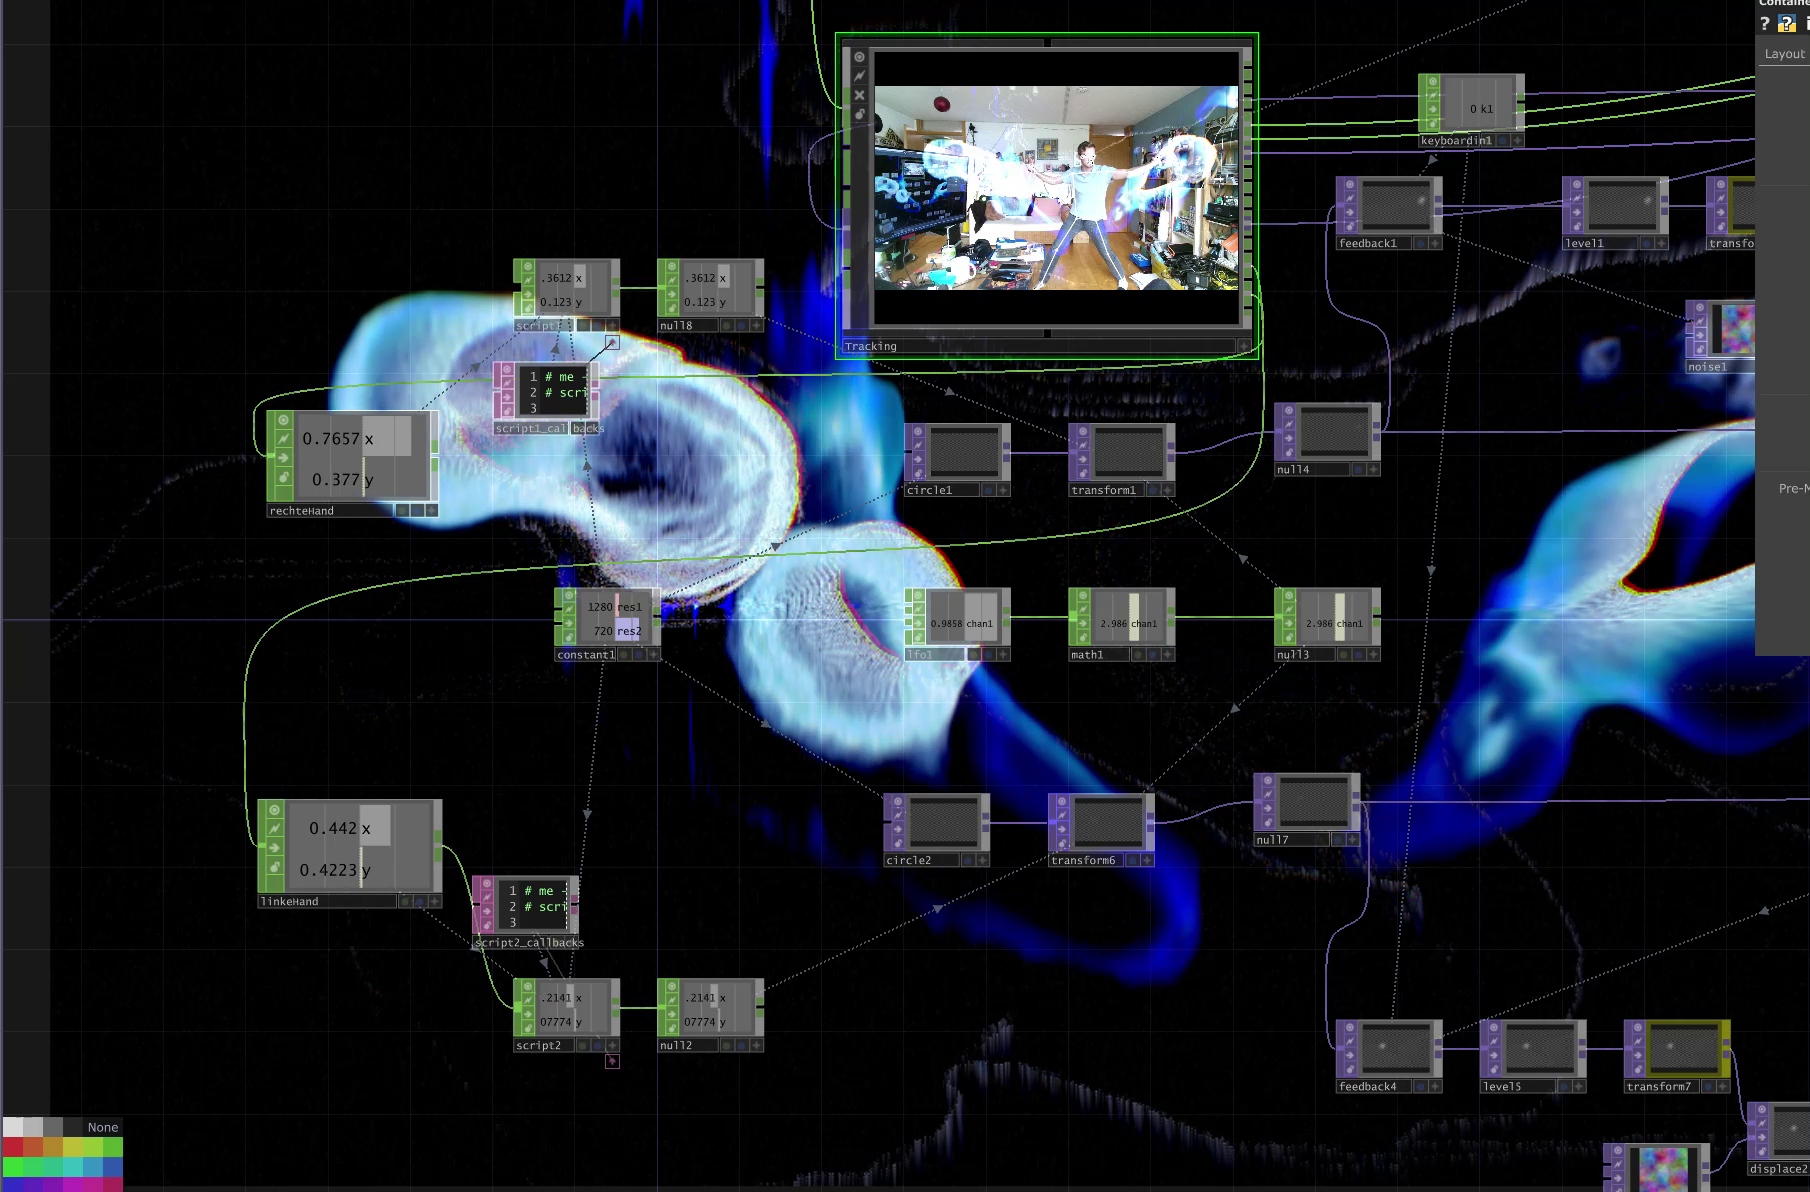
\includegraphics{images/docupictures/DemonstrationOfTheMagicalFireHands.png}%
    }
    \caption{Live-Demonstration des NoisyBlob Hand-Feuer-Effekts bei mir im Test-Setup zuhause: Blaue Partikel-Emission folgen den Händen}
    \label{fig:handfeuer_demonstration}
\end{figure}

\begin{figure}[htbp]
    \centering
    \adjustbox{max width=0.8\textwidth, max height=0.8\textheight, keepaspectratio}{%
        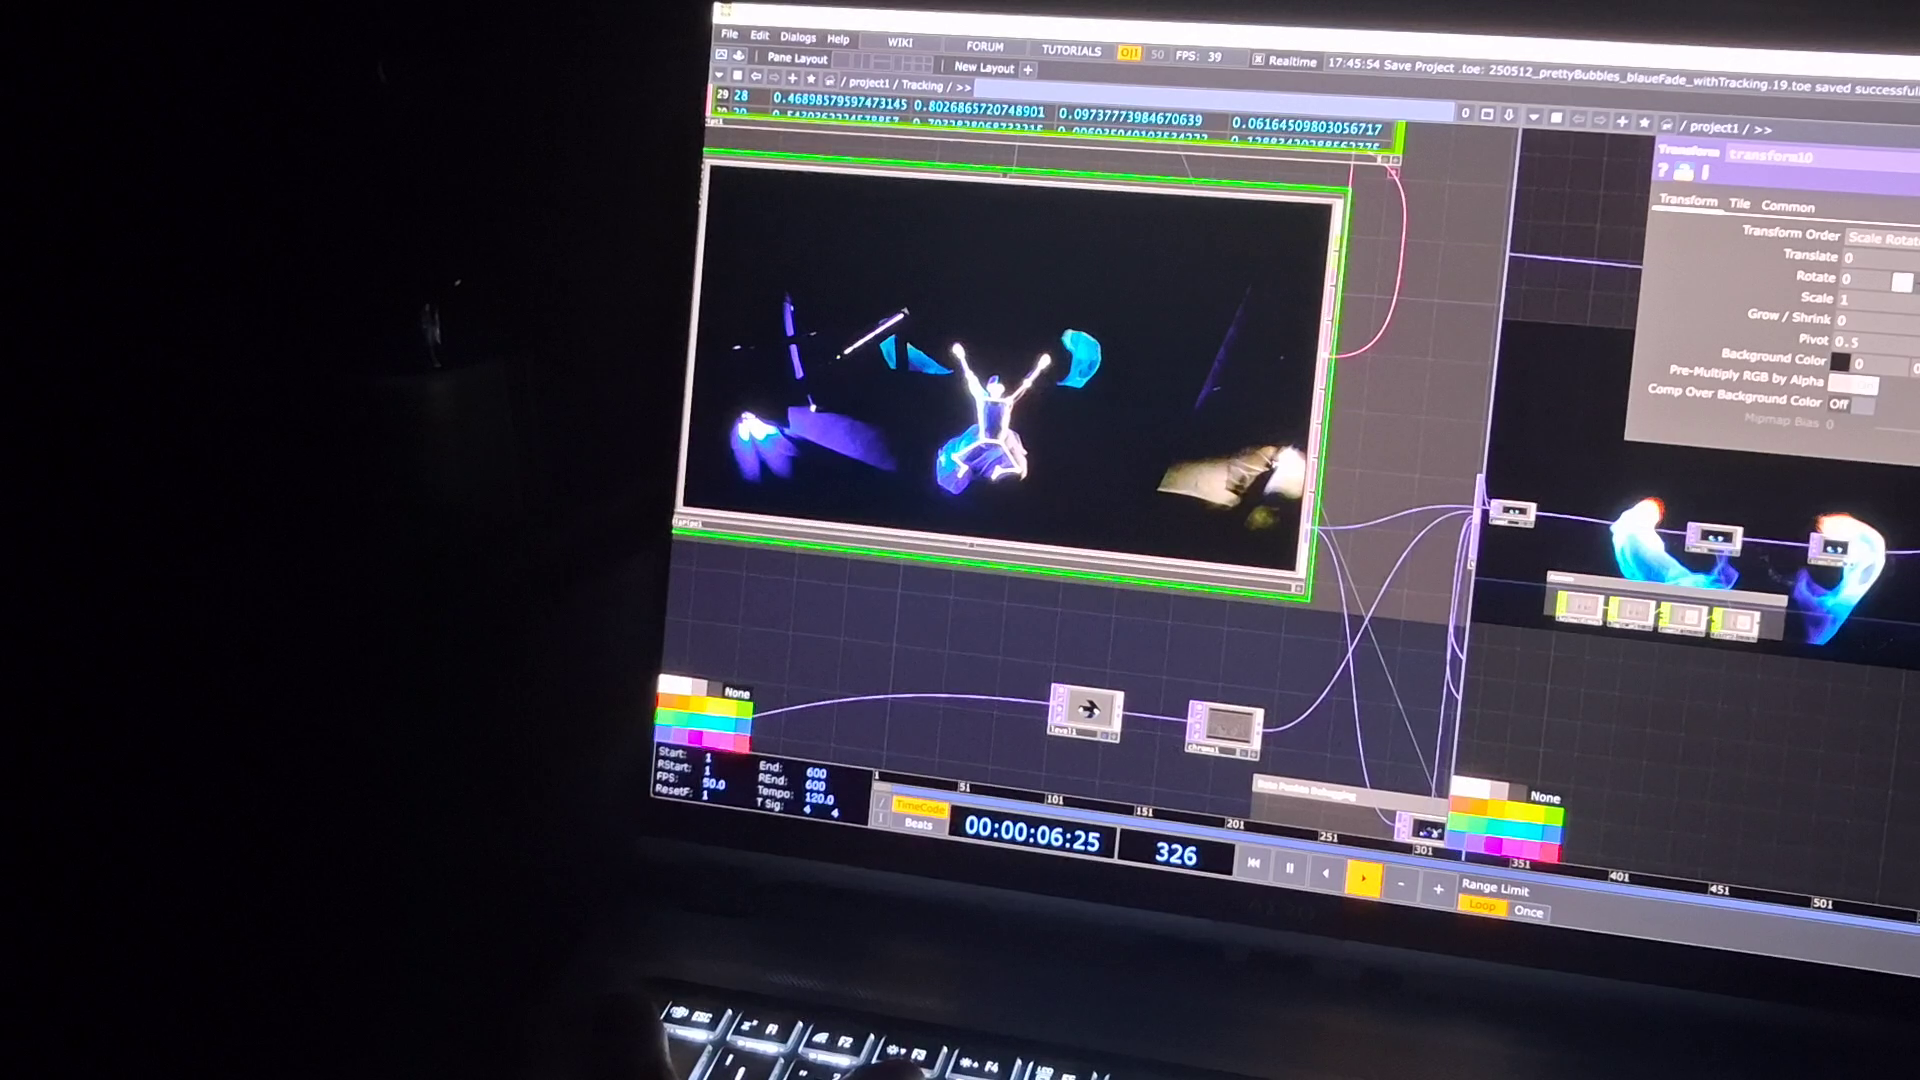
\includegraphics{images/onSetImages/dancerWithHandFireViewFromKinect.png}%
    }
    \caption{Hand-Feuer in Aktion, Sicht aus TouchDesigner: Blaue Partikel folgen den Händen. Gut zu erkennen ist das MediaPipe-Skelett, dass auch die nicht sichtbaren Füße predicted.}
    \label{fig:hand_fire_action}
\end{figure}

\textbf{Visual-System 2: Adaptive Kopfpartikel}

Die Kopfpartikel-Implementation verwendet eine Zustandsmaschine mit zwei Modi. Der Wechsel erfolgt durch Vergleich der Y-Koordinaten von Hand- und Schulter-Nodes. Eine Interpolationsfunktion sorgt für sanfte Übergänge zwischen den Zuständen. Die frontale Ausrichtung erfordert präzise Kalibrierung der Beamer-Kamera-Relation.

\begin{figure}[htbp]
    \centering
    \adjustbox{max width=0.9\textwidth, max height=0.8\textheight, keepaspectratio}{%
        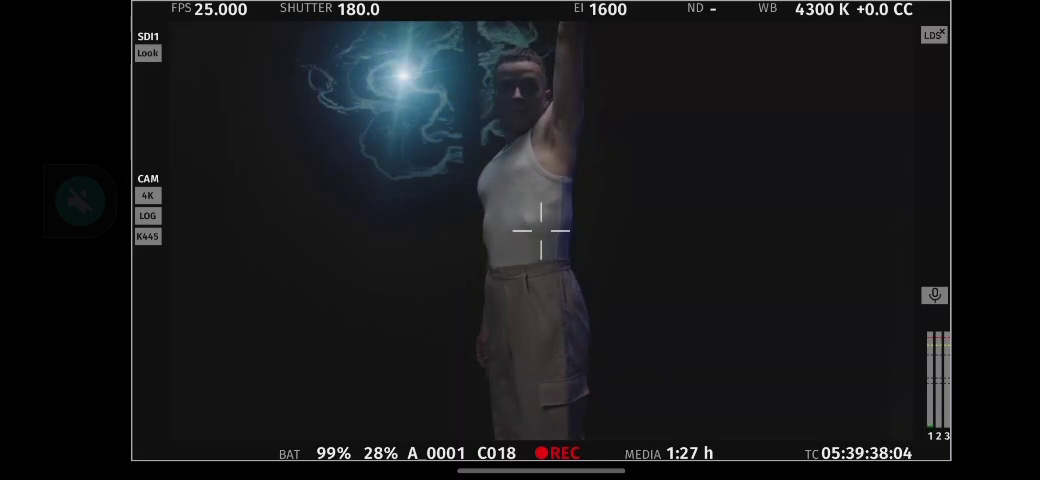
\includegraphics{images/onSetImages/HeadTrackingLeftSideOfHeadWithHeadClearlyAttached.png}%
    }
    \caption{Head-Tracking Perspektive mit seitlichem Blickwinkel. Die Blobs sind präzise am Kopf des Performers angebracht}
    \label{fig:low_light_tracking}
\end{figure}

\begin{figure}[htbp]
    \centering
    \adjustbox{max width=0.8\textwidth, max height=0.8\textheight, keepaspectratio}{%
        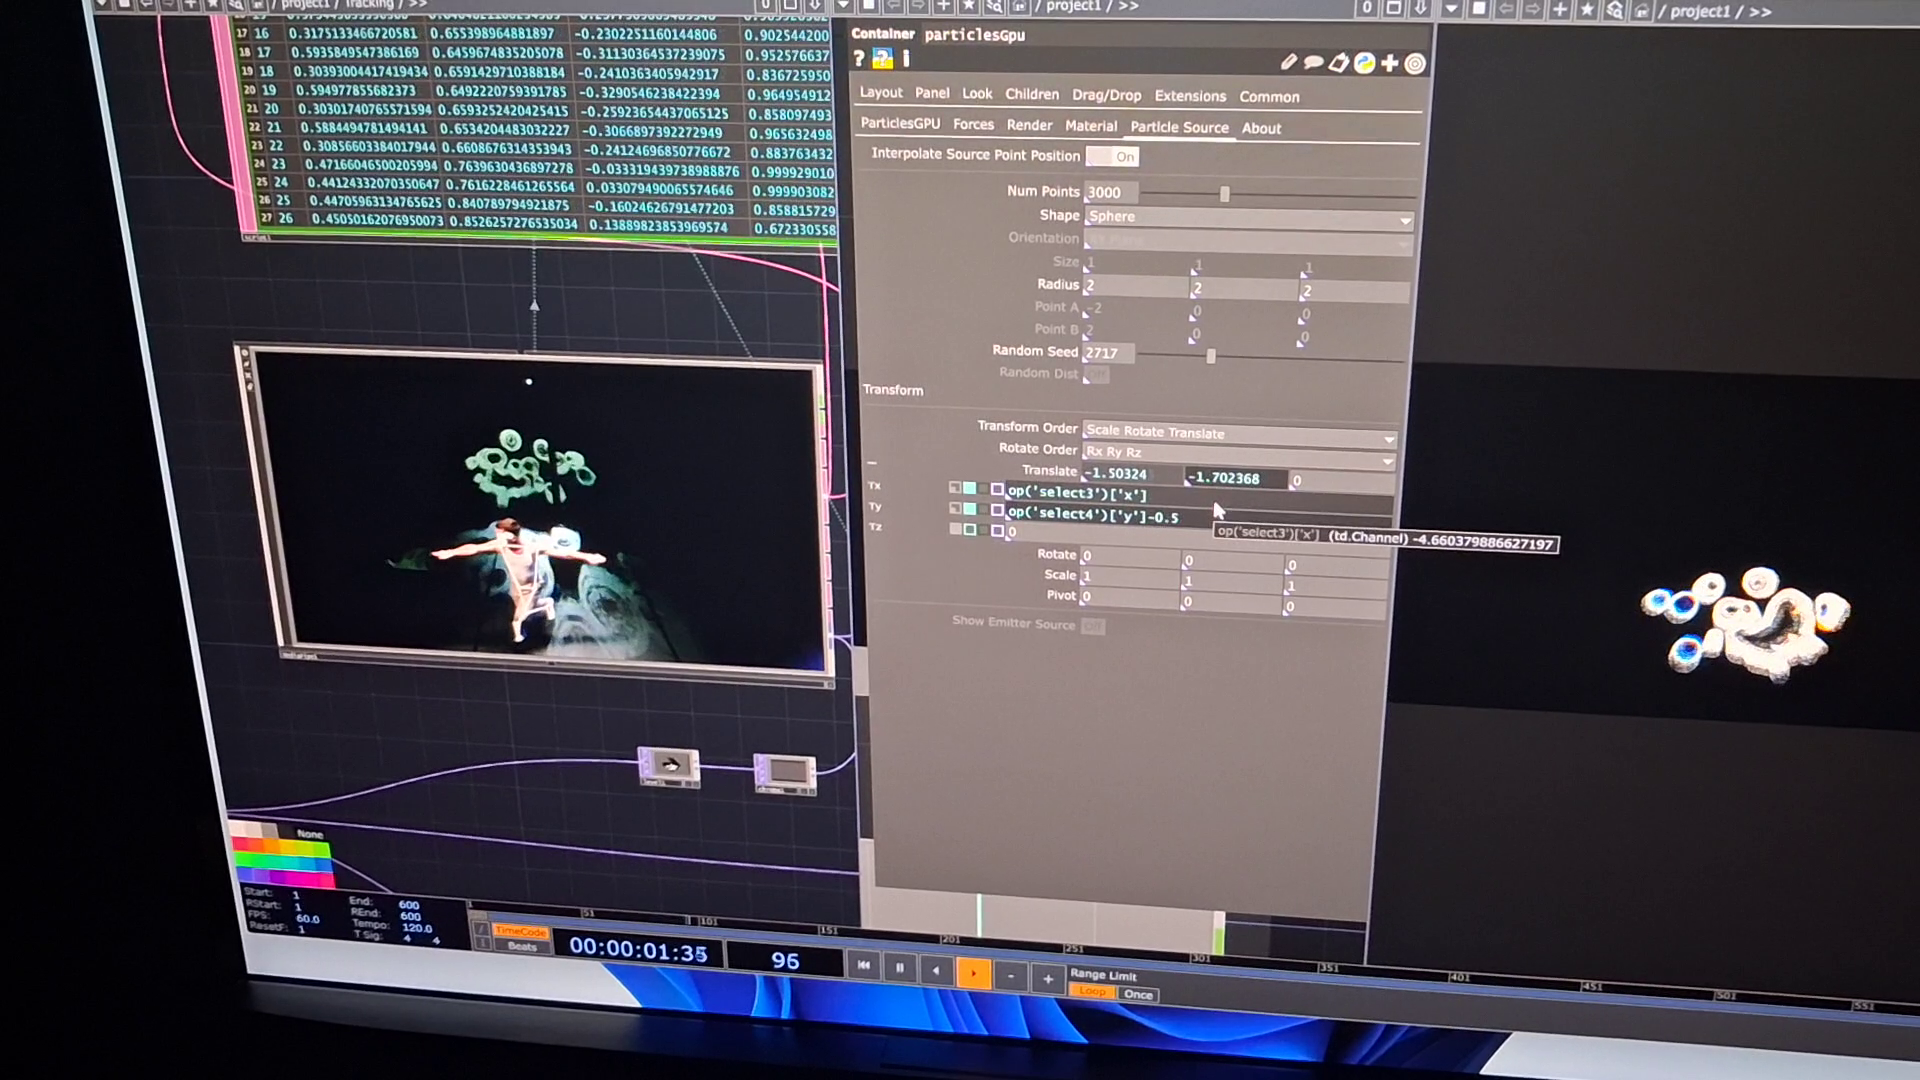
\includegraphics{images/onSetImages/HeadtrackingBubblesClearlyAtHeadLevelOnBackgroundBeamerMediaPipeSkeletonBeautifullyVisible.png}%
    }
    \caption{TouchDesigner und Kinect Perspektive: Head-Tracking-Bubbles Endergebnis: MediaPipe-Skelett-Erkennung mit Beamer-Projektion trotz Herausforderungen erfolgreich}
    \label{fig:head_result}
\end{figure}

\begin{figure}[htbp]
    \centering
    \adjustbox{max width=0.9\textwidth, max height=0.8\textheight, keepaspectratio}{%
        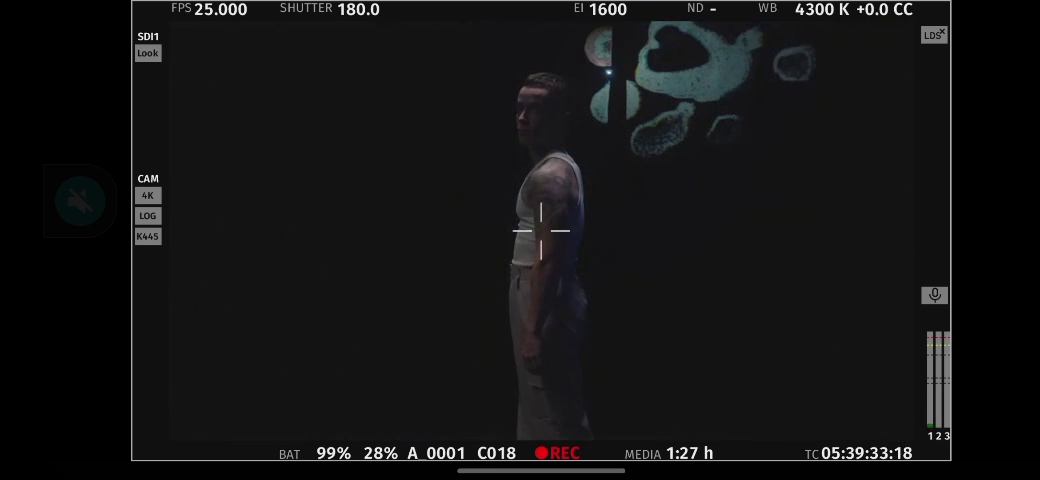
\includegraphics{images/onSetImages/HQCameraHeadtrackingVisibleWithBubblesOffsetCorrectlyFromHQCameraViewToAppearOnRightSideOfHead.png}%
    }
    \caption{HQ-Kameraperspektive: Kopfpartikel mit korrektem Offset zur rechten Seite des Performers für präzise Beamer-Projektion}
    \label{fig:headtracking_hq_kamera_offset}
\end{figure}

\textbf{Visual-System 3: 64-Spike Radialsystem}

Das Spike-System berechnet Polarkoordinaten der Hand- und Fußpositionen relativ zum Bildschirmzentrum. Der atan2-Algorithmus mappt Winkel auf diskrete Spike-Indizes (0-63). Die Spike-Intensität korreliert mit der Distanz zum Zentrum. Das System arbeitet mit Top-Down-Perspektive und Infrarot-Tracking für hohe Stabilität.

\begin{figure}[htbp]
    \centering
    \adjustbox{max width=0.8\textwidth, max height=0.8\textheight, keepaspectratio}{%
        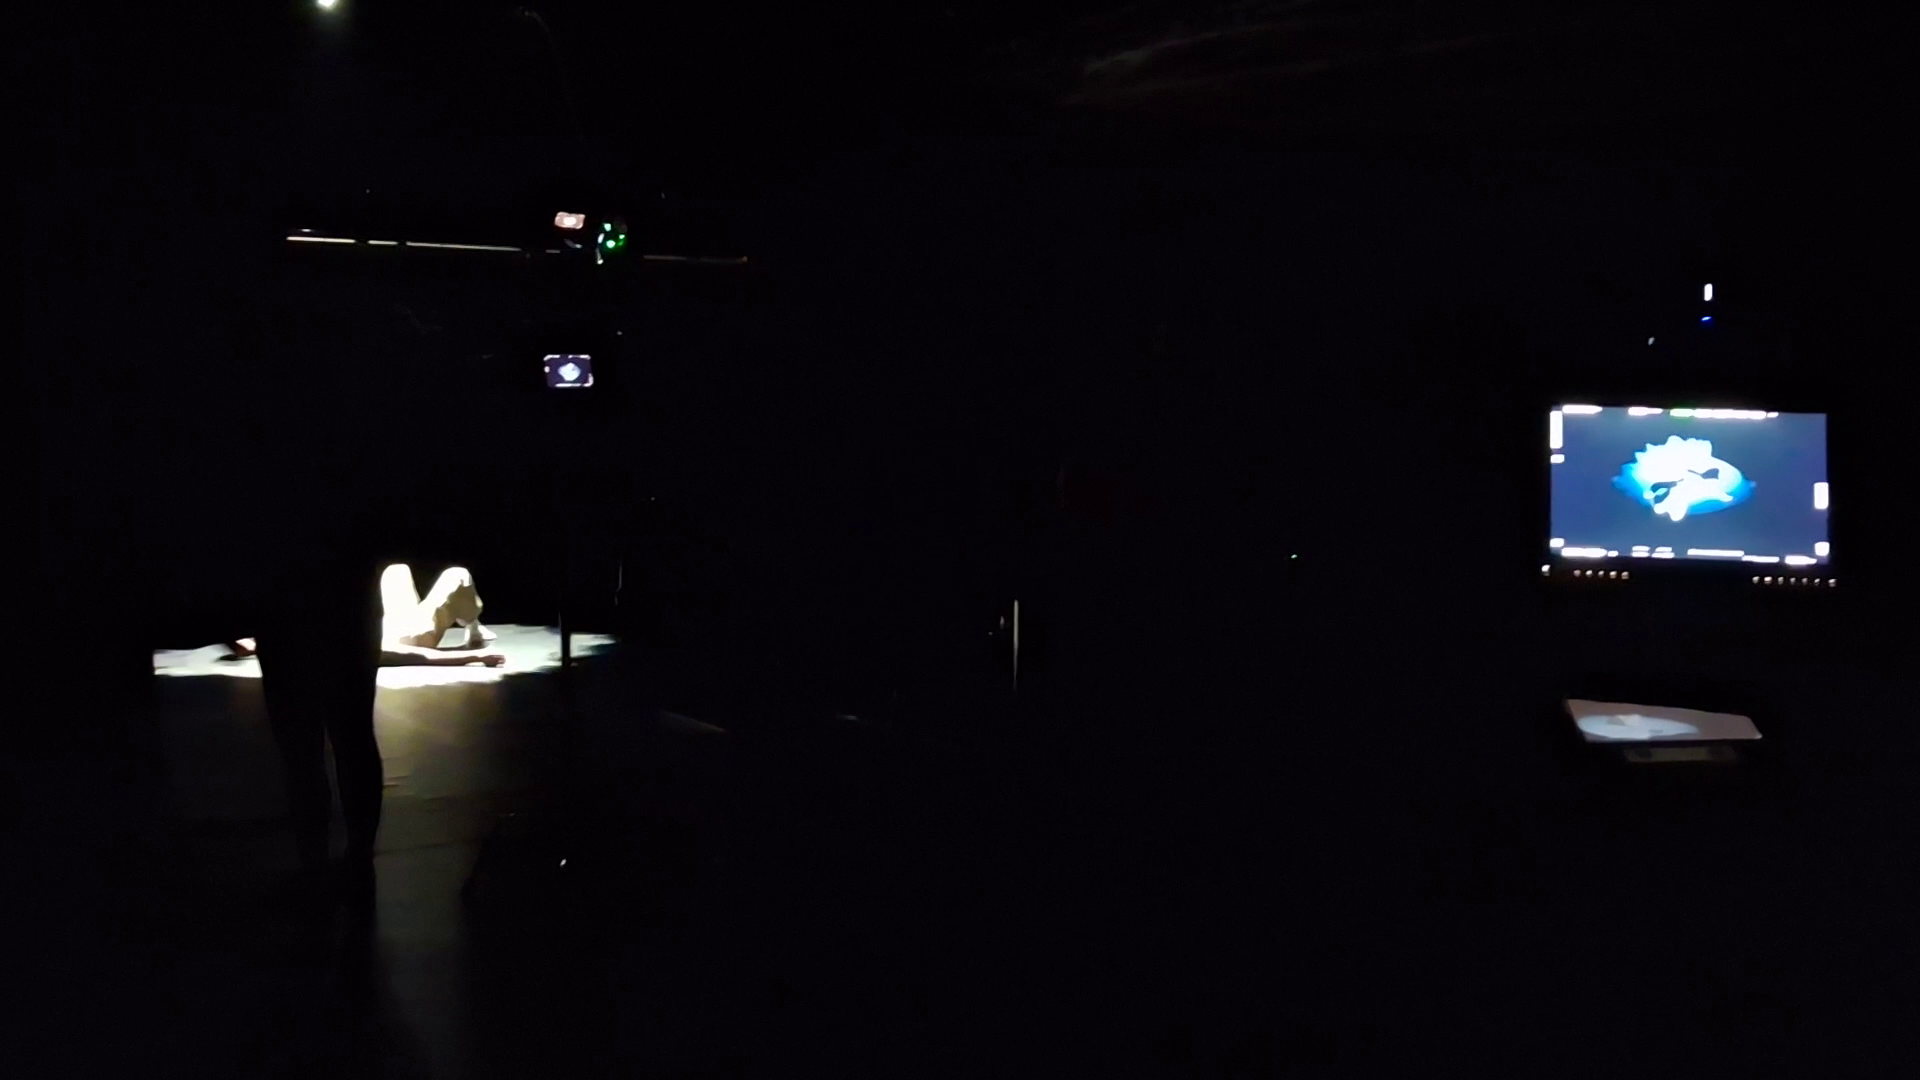
\includegraphics{images/onSetImages/BTS_TopDown_DancerAndProducer.png}%
    }
    \caption{Behind the Scenes: Tänzer mit professioneller Lichttechnik und Producer-Ansicht beim Top-Down-Shot}
    \label{fig:studio_wide}
\end{figure}

\clearpage
\subsection{Infrarot-Tracking-Pipeline}


Die zentrale Lösung besteht in der Weiterleitung des Kinect V2 Infrarot-Streams über OBS Virtual Camera an MediaPipe. Diese Lösung umgeht Beleuchtungsinterferenzen durch Beamer-Projektionen. Der IR-Stream wird in Echtzeit zu Grayscale konvertiert und als virtuelle Kamera bereitgestellt.

\subsection*{Datenverarbeitungs-Pipeline}


Die Datenverarbeitung erfolgt durch sieben spezialisierte Python-Skripte:

\begin{itemize}
    \item \texttt{PY\_MediaPipeDebugCirclesForCompTops.py}: Visualisiert Tracking-Confidence
    \item \texttt{PY\_NodeXYzuCentralisedSOPTranslate.py}: Koordinatensystem-Transformation
    \item \texttt{PY\_NodeToParticleGPUtranslate.py}: Hand-zu-Partikel-Mapping
    \item \texttt{PY\_AngleToPhaseSkript\_HandsToCenter\_direct.py}: Spike-Berechnung
    \item \texttt{PY\_RelativeNodeValuesToBlended0and1Switch.py}: Zustandslogik
    \item \texttt{PY\_NodeDatsToDistanceAngles.py}: Geometrische Relationen
    \item \texttt{PY\_OG\_TestingWithSynchAndKalman.py}: Legacy-Referenz
\end{itemize}

\subsection*{Performance-Charakteristika}


Das System erreicht folgende Performance-Metriken:
\begin{itemize}
    \item \textbf{Ende-zu-Ende-Latenz:} Sehr niedrig mit konstanter Bildrate
    \item \textbf{Tracking-Präzision:} Sehr hoch (IR-Modus), gut (RGB-Modus)
    \item \textbf{CPU-Auslastung:} 23\% (optimiert von initial 85\%)
    \item \textbf{GPU-Auslastung:} 45\% bei allen drei Systemen parallel
    \item \textbf{Speicherbedarf:} Moderater Arbeitsspeicher
\end{itemize}

\subsection*{Installation und Deployment}

Repository: \url{https://github.com/mklemmingen/MASK}

Systemanforderungen:
\begin{itemize}
    \item Windows 10/11 (64-bit)
    \item TouchDesigner 2023.11760 oder höher
    \item Kinect V2 mit offiziellen Treibern
    \item OBS Studio 28.0+ mit Virtual Camera
    \item Ausreichend Arbeitsspeicher
\end{itemize}

Die Installation erfolgt durch Klonen des Repositories und Import der .tox-Dateien in TouchDesigner. Die modulare Struktur ermöglicht selektive Integration einzelner Komponenten.